\documentclass[12pt]{article}
\usepackage[T1, T2A]{fontenc}
\usepackage[utf8]{inputenc}
\usepackage[russian]{babel}
\usepackage{hyperref}
\usepackage{graphicx}
\graphicspath{ {../Images/} }

\author{Григорий Матюхин}
\date{\today}
\title{Лабораторная работа \textnumero11.\\Управление загрузкой системы}

\begin{document}
\maketitle
\newpage
\tableofcontents
\newpage
\section{Цель работы}
Получить навыки работы с загрузчиком системы GRUB2.

\section{Последовательность выполнения работы}

\subsection{Модификация параметров GRUB2}
\begin{enumerate}
	\item Запустите терминал и получите полномочия администратора:
	\item В файле \texttt{/etc/default/grub} удалите параметры \texttt{rhgb} и \texttt{quiet} из строки указания параметров запуска ядра системы:
	\item В этом же файле установите параметр отображения меню загрузки в течение 10 секунд:
	      \\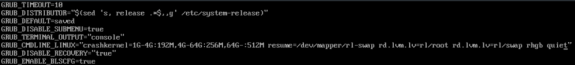
\includegraphics{1.png}
	\item Запишите изменения в GRUB2:
	      \\
\includegraphics{2.png}
	\item Перезагрузите систему и убедитесь, что при загрузке вы видите прокрутку загрузочных сообщений:
\end{enumerate}

\subsection{Устранения неполадок}
\begin{enumerate}
	\item Запустите (перегрузите) систему. Как только появится меню GRUB, выберите строку с текущей версией ядра в меню и нажмите \texttt{e} для редактирования:
	\item Прокрутите вниз до строки, начинающейся с \texttt{linux (\$root)/vmlinuz-}.
	      В конце этой строки введите \texttt{systemd.unit=rescue.target} и удалите опции \texttt{rhgb} и \texttt{quiet} из этой строки, если они там есть:
	      \\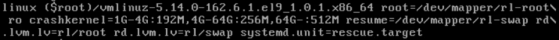
\includegraphics{3.png}
	\item Нажмите \texttt{Ctrl + x} для продолжения процесса загрузки:
	\item Введите пароль пользователя \texttt{root} при появлении запроса:
	      \\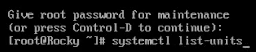
\includegraphics{4.png}
	\item Посмотрите список всех файлов модулей, которые загружены в настоящее время:
	      \\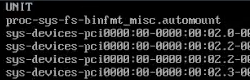
\includegraphics{5.png}
	\item Посмотрите задействованные переменные среды оболочки:
	      \\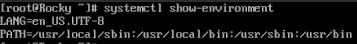
\includegraphics{6.png}
	\item Перегрузите систему.
	\item Как только отобразится меню GRUB, ещё раз нажмите \texttt{e} на строке с текущей версией ядра, чтобы войти в режим редактора. В конце строки, загружающей ядро, введите \texttt{systemd.unit=emergency.target}:
	      \\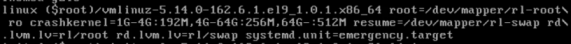
\includegraphics{7.png}
	\item Нажмите \texttt{Ctrl + x} для продолжения процесса загрузки.
	\item Введите пароль пользователя root при появлении запроса:
	      \\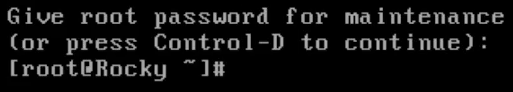
\includegraphics{8.png}
	\item После успешного входа в систему посмотрите список всех загруженных файлов модулей:
	      \\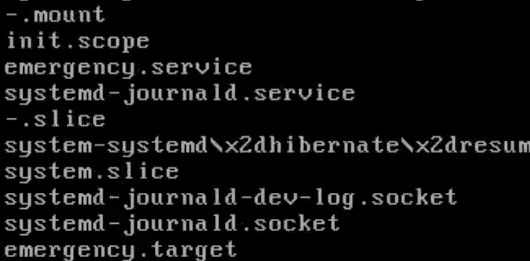
\includegraphics{9.png}
	\item Перегрузите систему.
\end{enumerate}

\subsection{Сброс пароля \texttt{root}}
\begin{enumerate}
	\item Запустите (перегрузите) компьютер. Когда отобразится меню GRUB, выберите в меню строку с текущей версией ядра системы и нажмите \texttt{e}, чтобы войти в режим редактора.
	      В конце строки, загружающей ядро, введите \texttt{rd.break} и удалите опции \texttt{rhgb} и \texttt{quiet} из этой строки, если они там есть:
	      \\
\includegraphics{10.png}
	\item Нажмите \texttt{Ctrl + x} для продолжения процесса загрузки:
	\item Чтобы получить доступ к системному образу для чтения и записи, наберите \texttt{mount -o remount,rw /sysroot}:
	\item Сделайте содержимое каталога \texttt{/sysroot} новым корневым каталогом:
	      \\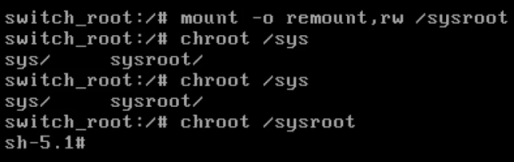
\includegraphics{11.png}
	\item Теперь вы можете ввести команду задания пароля и установить новый пароль для пользователя \texttt{root}:
	      \\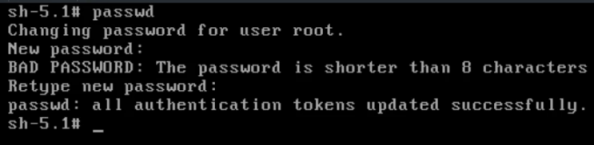
\includegraphics{12.png}
	\item Загрузите политику SELinux:
	      \\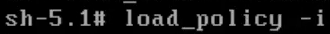
\includegraphics{13.png}
	\item Установите правильный тип контекста для \texttt{/etc/shadow}:
	      \\
\includegraphics{14.png}
	\item Перезагрузите систему и войдите в систему с изменённым паролем для пользователя \texttt{root}:
	      \\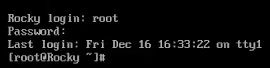
\includegraphics{15.png}
\end{enumerate}

\section{Контрольные вопросы}
\begin{enumerate}
	\item Какой файл конфигурации следует изменить для применения общих изменений в GRUB2? \\
	      \texttt{/etc/default/grub}
	\item Как называется конфигурационный файл GRUB2, в котором вы применяете изменения для GRUB2? \\
	      \texttt{/boot/grub/grub.cfg}
	\item После внесения изменений в конфигурацию GRUB2, какую команду вы должны выполнить, чтобы изменения сохранились и воспринялись при загрузке системы? \\
	      \texttt{grub2-mkconfig > /boot/grub/grub.cfg}
\end{enumerate}

\section{Вывод}
В ходе выполнения данной работы я получил навыки работы с загрузчиком системы GRUB2.

\end{document}
